<<<<<<< HEAD
\section{IrvanRizkiansyah/1174043}
	\subsection{Pemahaman Teori}
		\begin{enumerate}
			\item \begin{itemize}
					\item Fungsi : File csv berfungsi untuk pencarian data akan menjadi lebih mudah dan cepat, dan juga mempermudah penginputan data ke dalam database secara sederhana.
					\item Sejarah : File csv muncul pertama kali sekitar 10 tahun sebelum Personal Computer (PC) pertama  didunia yaitu sejak sekitar tahun 1972, akan tetapi sebutan file csv digunakan pertama kali pada tahun 1983.
					\item Contoh : 
						\begin{figure} [ht]
							\centerline{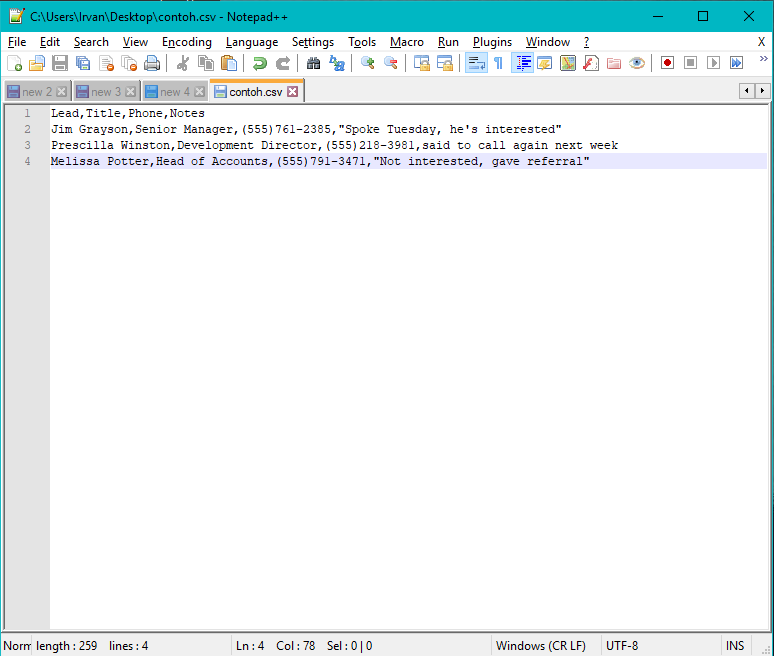
\includegraphics[width=0.6\textwidth]{figures/chapter4/Contoh_CSV.png}}
							\caption{Contoh CSV}
							\label{Contoh CSV}
						\end{figure}

					\ref{Contoh_CSV}
				\end{itemize}
			
			\item Ada banyak aplikasi yang dapat membuat file berformat CSV, diantaranya adalah :
				\begin{itemize}
					\item Notepad
					\item Notepad++
					\item Microsoft Excel
					\item Corel Quatro Pro
					\item Apache Open Office, dan masih banyak yang lainnya.
				\end{itemize}
			
			\item Cara menulis file csv menggunakan Excel :
				\begin{enumerate}
					\item Buka aplikasi Microsoft Excel kemudian buat dokumen baru
					\item Tulis judul kolom untuk setiap informasi yang ingin di rekam atau catat, kemudian tulis informasi - informasi dalam kolom dengan sesuai.
					\item Jika sudah selesai maka save dengan cara pilih menubar File lalu pilih Save As
					\item Lalu isikan nama file tersebut dan rubah dengan memilih format file yang tersedia tersebut menjadi .csv
					\item File csv sudah berhasil terbuat menggunakan Microsoft Excel
				\end{enumerate}
			\item Cara membaca file csv menggunakan Excel :
				\begin{enumerate}
					\item Buka aplikasi Microsoft Excel kemudian pilih menu Open
					\item Cari tempat file csv yang ingin dibuka, kemudian pilih Open
					\item File csv sudah berhasil dibaca menggunakan Microsoft Excel
				\end{enumerate}
			
			\item Pada file csv, tanda baca koma diartikan sebagai pembatas suatu kolom. List-directed input output didefinisikan dalam FORTRAN 77. List-directed input menggunakan tanda baca koma atau spasi sebagi pembatas, sehinnga karakter yang tidak dikutip tidak dapat mengandung tanda baca koma ataupun spasi. Hal tersebut yang diadopsi oleh file csv. format csv didukung dengan library untuk banyak bahasa pemrograman, kebanyakan yang menspesifikasikan pembatas field, pemisah desimal, pengkodean karakter, dan yang lainnya.
			
			\item Pada tahun 2008, pengembangan pandas dimulai oleh AQR Capital Management. Pada akhir tahun 2009 pandas menjadi Open Sourced, dimana disupport oleh banyak komunitas atau individu di dunia untuk mengembangkan pandas. Sejak tahun 2015, pandas menjadi NumFOCUS proyek sponsor, ini juga membantu suksesnya pengembangan dari pandas itu sendiri. pandas merupakan struktur data dan data analysis tools untuk bahasa pemrograman Python, dan merupakan BSD-licensed library yang menjadikannya memiliki performa yang tinggi.
			
			\item 
				\begin {itemize} 
					\item Tanda baca koma : Menjadi pemisah antar kolom
					\item Tanda baca kutip dua : Menjadi cara untuk memasukan sebuah kalimat atau untuk memasukan karakter spasi sebagai data pada kolom informasi
					\item Inputan pada baris pertama akan menjadi Header, dimana akan menjadi nama sebuah kolom, dan masih banyak yang lainnya
				\end{itemize}
			
			\item Pada pandas sedikit berbeda, dimana inputan data berbentuk seperti peng-inputan pada variabel pada umumnya, hanya saja menggunakan tanda kutip satu untuk menandakan sebuah informasi pada kolom kemudian tanda kurung kotak yang didalamnya berisi informasi data dari kolom tersebut. dan lain sebagainya.
			
		\end{enumerate}

\subsection{Luthfi Muhammad Nabil/1174035}
\subsubsection{Fungsi, Sejarah, dan Contoh file CSV}
\begin{itemize}
	\item Fungsi \linebreak File CSV (Comma Separated Values) adalah tipe file khusus yang menyimpan informasi dengan metode dipisahkan dengan koma. File CSV berfungsi untuk menjadi perantara untuk beberapa aplikasi yang memiliki basis data saat mengirim data. CSV dapat dibuka di berbagai text editor
	yang ada. Dengan bentuk filenya yang dinamis memungkinkan file CSV dapat dimanipulasi dan dapat menyimpan informasi dengan skala besar.
	\item Sejarah \linebreak CSV sudah digunakan sejak tahun 1972 yang dapat dikompilasi pada bahasa pemrograman IBM Fortran. Saat itu, data yang dipisahkan oleh koma jika isinya memiliki spasi maka harus diberi tanda petik di awal dan akhir isi dari data tersebut. Nama CSV baru mulai digunakan pada tahun 1983. Pada panduan dari Osborne Executive Computer mendokumentasikan kutipan yang membolehkan isi karakter memiliki koma.  Pada tahun 2005 dengan RFC4180, CSV didefinisikan sebagai MIME Content Type. lalu pada tahun 2013, defisiensi dari RFC4180 dipecahkan oleh rekomendasi dari W3C. Pada tahun 2014, IETF mempublikasi RFC7111 yang mendeskripsikan pecahan Uniform Resource Identifier(URI) ke dokumen CSV. RFC7111 menjelaskan bagaimana baris, kolom dapat dipilih dalam dokumen CSV menggunakan indeks posisi. Pada Tahun 2015, W3C mempublikasikan draft rekomendasi untuk CSV-metadata standards yang dimulai dengan rekomendasi pada bulan Desember dengan tahun yang sama. 
	\item Contoh File CSV \begin{itemize}
							\item 
							CSV pada Excel \ref{1174035_CSVExcel}
							\begin{figure}[!htbp]
								\centering
								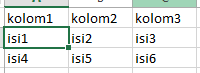
\includegraphics[height=4cm, width=7cm]{figures/chapter4/1174035_CSVExcel.jpg}
								\caption{Contoh CSV Pada Excel}
								\label{1174035_CSVExcel}
							\end{figure}
							\item \begin{figure}[!htbp]
								\centering
								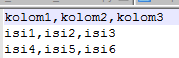
\includegraphics[height=4cm, width=7cm]{figures/chapter4/1174035_CSVText.jpg}
								\caption{Contoh CSV Pada Text}
								\label{1174035_CSVText}
							\end{figure}
							CSV pada Text Editor \ref{1174035_CSVText}
							
						  \end{itemize}
\end{itemize}
\subsubsection{Aplikasi Yang dapat membuat file CSV}
Berikut file yang dapat membuat file CSV
\begin{itemize}
	\item Spreadsheet \linebreak Spreadsheet merupakan aplikasi yang dapat membuat CSV hanya dengan memasukan data sesuai baris dan kolom yang diinginkan. Contoh spreadsheet seperti Google Spreadsheet, Microsoft Excel, dan aplikasi lainnya. 
	\item Bahasa Pemrograman \linebreak Bahasa pemrograman merupakan media yang dapat untuk membuat aplikasi yang dapat membuat file CSV khusus untuk bahasa pemrograman yang support dengan pembuatan file CSV. Seperti Python, C Sharp, dan lain sebagainya.
	\item Text Editor \linebreak Text editor juga dapat membuat file CSV, untuk membuat dengan Text Editor cukup dengan membuat file sesuai format CSV dan save file tersebut dengan ekstensi .CSV.
\end{itemize}
\subsubsection{Menulis dan Membaca file CSV}
Berikut cara menulis dan membaca file CSV : 
\begin{itemize}
	\item Menulis : \begin{enumerate}
						\item Buka file CSV dengan spreadsheet
						\item Klik Cell yang mau diisi
						\item Masukan data yang mau diisi pada cell tersebut
						\item Lalu save file dengan format .CSV
					\end{enumerate}
	\item Membaca : \begin{enumerate}
						\item Buka file CSV dengan spreadsheet						
					\end{enumerate}
\end{itemize}
\subsubsection{Sejarah Library CSV Python}
Library CSV pada python merupakan library yang paling umum untuk import export data pada spreadsheet dan basis data dengan format sesuai dengan standarisasi RFC4180. Seiring dengan lahirnya bahasa pemrograman python, library mulai dibuat dan dikembangkan sampai akhirnya pada tahun 2003, pembuatnya Kevin Altis dan lainnya telah merilis versi final untuk library Python CSV. 
\subsubsection{Sejarah Library Pandas Python}
Pandas (Python Data Analysis Library) adalah library open source yang digunakan untuk melakukan data manajemen dan data analysis. Pandas diciptakan pada tahun 2008 oleh Wes McKinney dan diperbaharui oleh Sien Chang pada tahun 2010. Inspirasi dari pembuatan pandas muncul pada komunitas yang membutuhkan library khusus untuk analisis data. 
\subsubsection{Fungsi - fungsi yang terdapat di library CSV}
\begin{itemize}
	\item \begin{verbatim} csv.reader(csvfile, dialect='excel', **fmtparams) \end{verbatim} Untuk mengembalikan	object reader yang akan mengambil setiap line pada csv yang diambil. Data setiap baris diambil saat next() dipanggil. Berikut contohnya : \lstinputlisting[firstline=1, lastline=6]{src/chapter4/chap4_1174035_teori.py}
	\item \begin{verbatim} csv.writer(csvfile, dialect='excel', **fmtparams) \end{verbatim} Mengembalikan file pembuat object untuk dapat mengkonversi data pada python ke file CSV yang akan dibuat. Berikut contoh penggunaan csv.writer : \lstinputlisting[firstline=8, lastline=14]{src/chapter4/chap4_1174035_teori.py}
	\item \begin{verbatim} csv.register_dialect(name[, dialect[, **fmtparams]]) \end{verbatim} Mengasosiasikan dialek dengan nama, nama yang dimasukkan harus berupa karakter.
	\item \begin{verbatim} csv.unregister_dialect(name) \end{verbatim}
	Menghapus asosiasi dialek dengan nama pada registry dialek.
	\item \begin{verbatim} csv.get_dialect(name) \end{verbatim}
	Mengambil dialek yang telah diasosiasikan dengan nama. 
	\item \begin{verbatim}  csv.list_dialects() \end{verbatim} Mengembalikan dialek yang telah diregistrasi.
	\item \begin{verbatim} csv.field_size_limit([new_limit]) \end{verbatim} Mengembalikan maksimal kolom data yang diperbolehkan oleh pembaca.
\end{itemize}
\subsubsection{Fungsi - fungsi yang terdapat di library Pandas}
\begin{itemize}
	\item \begin{verbatim} pandas.read_csv(filepath_or_buffer[, sep, …]) \end{verbatim} Untuk membaca file CSV dan menyimpannya ke DataFrame
	\item \begin{verbatim} pandas.read_excel(io[, sheet_name, header, names, …])  \end{verbatim} Membaca file excel dan menyimpannya ke DataFrame
	\item \begin{verbatim} to_csv([path, index, sep, na_rep, …]) \end{verbatim}
	Untuk membuat file CSV dari data yang ada	
\end{itemize}
=======
\section{Faisal Najib Abdullah}
\subsection{Pemahaman Teori}
\begin{enumerate}
    \item Apa itu fungsi file csv, jelaskan sejarah dan contoh ?
    \par
    File CSV Nilai Berbatas Koma adalah tipe file khusus yang dapat Anda buat atau edit di Excel. File CSV menyimpan informasi yang dipisahkan oleh koma, bukan menyimpan informasi dalam kolom. Saat teks dan angka disimpan dalam file CSV, mudah untuk memindahkannya dari satu program ke program lain.
    \par 
	File CSV dibuat oleh program yang menangani sejumlah data yang besar. CSV merupakan cara yang nyaman untuk mengekspor data dari spreadsheet dan basis data serta mengimpor atau menggunakannya dalam program lain. Misalnya, Anda dapat mengekspor hasil program penambangan data ke file CSV dan kemudian mengimpornya ke dalam spreadsheet untuk menganalisis data, menghasilkan grafik untuk presentasi, atau menyiapkan laporan untuk publikasi.
    \par
	Contohnya, Anda dapat mengekspor kontak dari Google ke dalam file CSV, kemudian mengimpornya ke Outlook.
    
    \item Aplikasi-aplikasi apa saja yang bisa menciptakan file csv?
    Pada Windows
    \begin{itemize}
        \item Microsoft Excel 2013
        \item Microsoft Works
        \item CCorel Quattro Pro
        \item Apache OpenOffice
        \item LibreOffice
        \item Microsoft Notepad
        \item Intuit Quicken 2015
        \item GenScriber
    \end{itemize}
    Pada Mac OS
    \begin{itemize}
        \item Microsoft Excel 2011
        \item Planamesa NeoOffice
        \item Apache OpenOffice
        \item LibreOffice
        \item GenScriber
    \end{itemize}
    Pada Linux
    \begin{itemize}
        \item Apache OpenOffice
        \item LibreOffice
        \item GenScriber
    \end{itemize}
    
    \item Jelaskan bagaimana cara menulis dan membaca file csv di excel atau spreadsheet?
	\begin{itemize}
        \item Cara menulis file csv harus berupa baris dan kolom atau bisa juga di sebut berupa tabel.
        \item Untuk membacanya file csv dipisahkannya menggunakan koma atau titik koma.
    \end{itemize}
    
    \item Jelaskan sejarah library csv?
	Library csv menyediakan fungsionalitas untuk membaca dan menulis ke file CSV. Dirancang untuk bekerja di luar kotak dengan file CSV yang dihasilkan Excel, memudahkan untuk bekerja dengan berbagai format CSV. Library csv berisi objek dan kode lain untuk membaca, menulis, dan memproses data ke file CSV.
    
    \item Jelaskan sejarah library pandas?
	panda adalah pustaka Python open-source yang menyediakan alat analisis data kinerja tinggi dan struktur data yang mudah digunakan. panda tersedia untuk semua instalasi Python, tetapi itu adalah bagian penting dari distribusi Anaconda dan bekerja sangat baik di notebook Jupyter untuk berbagi data, kode, hasil analisis, visualisasi, dan teks naratif.

    \item Jelaskan fungsi-fungsi yang terdapat di library csv?
	Terdapat 2 fungsi yang bisa digunakan oleh library csv
    Pertama,fungsi membaca file csv.
    fungsi ini bisa menggunakan list dan dictionary
    Dengan list :
    \lstinputlisting[firstline=11, lastline=21]{src/chapter4/1174042_csv.py}
    Dengan dictionary :
    \lstinputlisting[firstline=24, lastline=33]{src/chapter4/1174042_csv.py}
    Kedua,fungsi menulis file csv.
    \lstinputlisting[firstline=36, lastline=40]{src/chapter4/1174042_csv.py}
    
    \item Jelaskan fungsi-fungsi yang terdapat di library pandas
	Hampir sama dengan library csv,tp library pandas penulisannya lebih sederhana dan terlihat lebih rapih dari pada library csv.
    \lstinputlisting[firstline=43, lastline=44]{src/chapter4/1174042_csv.py}
    

\end{enumerate}
>>>>>>> c64ab529ff89ebc66e82900d0611abe5d2422d5a
